\chapter{Tinker-Toy Project}
\section{The Boltzmann factor}
I could stop at this point. However, I wasn't quite satisfied with how idealistic my simulation was. Looking at the movement of each cell can be mesmerizing and seeing Brownian motion in action was quite a bit of fun. Yet, I knew it was incomplete. \par

\vspace{0.3cm}
To relax some of the assumptions, I decided to look back at rule 1 which states: 
\begin{enumerate}
    \item A cell can only be a 1 or 0.
\end{enumerate}
To model what's going on down there, there should be multiple levels of energy that are discrete by nature as Max Planck first proposed in order to solve the Ultraviolet catastrophe. Hence, I decided to tinker rule 1 to be as follows: 
\begin{itemize}
    \item A cell can have integer values between 0 to 8.
\end{itemize}
In this situation, a 0 cell represents the minimum amount of energy that a cell/particle can take or its ground state while an 8-cell represents the maximum amount of energy that a cell can take. \par

\vspace{0.3cm}
\noindent
This tweak adds a bit of realism to the simulation that changes the dynamics of how things work. After testing the prototype of version 2, I realized that a fundamental feature was missing, especially seeing that the clusters of heated particles had difficulty in dispersing their energy even at high move probabilities. To show what was wrong, we can look at the picture below to analyze the values. 
\begin{figure}[H]
\centering % center the figure
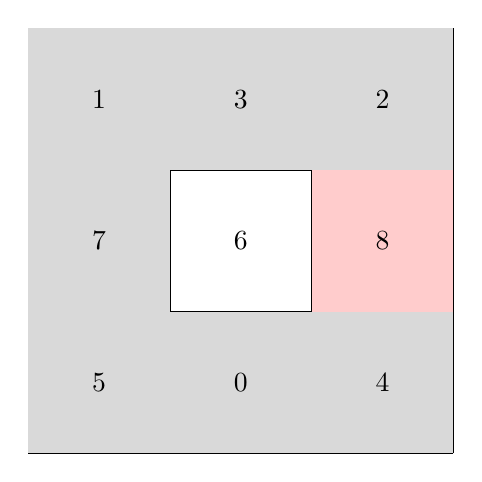
\begin{tikzpicture}[scale=1.8,minimum size=1.8cm]
    \draw (0,0) grid (3,3);
    \node at (0.5,2.5) [fill=gray!30] {1};
    \node at (1.5,2.5) [fill=gray!30] {3};
    \node at (2.5,2.5) [fill=gray!30] {2};
    \node at (0.5,1.5) [fill=gray!30] {7};
    \node at (1.5,1.5) {6};
    \node at (2.5,1.5) [fill=red!20] {8};
    \node at (0.5,0.5) [fill=gray!30] {5};
    \node at (1.5,0.5) [fill=gray!30] {0};
    \node at (2.5,0.5) [fill=gray!30] {4};
\end{tikzpicture}
\caption{\small {The cells that are colored are called the Moore neighborhood of the 6 cell}}
\label{fig:myfigure}
\end{figure}
In Figure \ref{fig:myfigure}, the shaded regions are the Moore neighborhood of the 6 cell located in the middle. As with version 1, the rules of movement was not altered for the prototype and 6 cell can transfer a unit of energy into any one of the grey cells with $\frac{1}{7}$ probability each. \par

\vspace{0.3cm}
\noindent
At this point, I knew the assumption of $\frac{1}{7}$ probability was wrong as in Chemistry, an electron will try to occupy the lowest energy state first rather than going into the higher orbitals. For instance, the way the electron goes toward orbitals is in the following order: ${1s^{2}, 2s^{2}, 2p^{6}, 3s^{2}, 3p^{6}, 4s^{2}, 3d^{10}, 4p^{6}}$. Hence, I needed some method or function that will modify the probabilities of each direction that is dependent on each cell's energy value. \par

\vspace{0.3cm}
\noindent
After some searching and reading articles on this topic, I came across the \href{https://en.wikipedia.org/wiki/Boltzmann_distribution}{Boltzmann factor} which conveniently addressed the problem quite well. The Boltzmann factor is given by: 
\vspace{0.2cm}
\begin{equation}
    \frac{p_{i}}{p_{j}}=e^{\dfrac{\epsilon_{j}-\epsilon_{i}}{kT}}
    \label{modboltz}
\end{equation}
The p terms represent the probability at state i and state j while the $\epsilon$ terms represent the energy at state j and i respectively. At this point, I wasn't exactly sure how to implement the Boltzmann factor to Figure \ref{fig:myfigure}. Since I wanted the simulation to make use of this concept, I decided to modify the Boltzmann factor into: 
\vspace{0.2cm}
\begin{equation}
    p_{j}=e^{\dfrac{8-\epsilon_{j}}{T}}
    \label{eq1}
\end{equation}
In this modified, version $\epsilon_{j}$ represents each cell's energy state within the Moore neighborhood and $p_{j}$ represents the probability that a unit of energy is transferred to that particular cell. \par

\vspace{0.3cm}
\noindent
Using this particular equation we can modify the probability that the 6 cell within Figure \ref{fig:myfigure} transfers its energy to each of the cells shaded grey. To do that we need to compute all of the probabilities and normalize them with a partition function. The partition function is defined as: 
\begin{equation}
    \sum_{j=1}^{\kappa} e^{\frac{8-\epsilon_{j}}{T}}
    \label{eq:2}
\end{equation}
Where $\kappa$ is the number of cells within the neighborhood excluding 8s. So for the picture in Figure \ref{fig:myfigure2}, $\kappa=7$ as we only have 7 "available cells" that the energy from the 6 cell can go to. \par

\vspace{0.3cm}
\noindent
Assuming that T=1, we can then divide each of Boltzmann's factors with \ref{eq:2}. This yields our probabilities of $P=[0.2330, 0.0315,0.0857, 0, 0.0116, 0.6333, 0.0043, 0.0006]$ for the cells labeled: $1, 3, 2, 8, 4, 0, 5, 7$ respectively. This means that there is a 61.6\% chance that the 6 cell within Figure \ref{fig:myfigure2} will send a unit of energy to a 0 cell and a 0.06\% chance that the 6 cell sends a unit of energy towards the 7 cell. \par

\vspace{0.3cm}
\noindent
To better depict the probabilities, I have made the picture below where each of the cell's values has a small text beside it which is the probability that a unit of energy from the 6 cell goes into the other cells. 
\begin{figure}[H]
\centering % center the figure
\begin{tikzpicture}[scale=1.8,minimum size=1.8cm]
    \draw (0,0) grid (3,3);
    \node at (0.5,2.5) [fill=gray!20] {1, \tiny{0.2330}} ;
    \node at (1.5,2.5) [fill=gray!20] {3, \tiny{0.0315}};
    \node at (2.5,2.5) [fill=gray!20] {2, \tiny{0.0857}};
    \node at (0.5,1.5) [fill=gray!20] {7, \tiny{0.0006}};
    \node at (1.5,1.5) {6};
    \node at (2.5,1.5) [fill=red!20] {8, \tiny{0}};
    \node at (0.5,0.5) [fill=gray!20] {5, \tiny{ 0.0043}};
    \node at (1.5,0.5) [fill=gray!20] {0, \tiny{ 0.6333}};
     \node at (2.5,0.5) [fill=gray!20] {4, \tiny{0.0116}};

    \draw [-stealth] ($(1.5,1.5)!0.4!(0.5,2.5)$) -- ($(1.5,1.5)!0.6!(0.5,2.5)$) ;
    \draw [-stealth] ($(1.5,1.5)!0.4!(1.5,2.5)$) -- ($(1.5,1.5)!0.6!(1.5,2.5)$) ;
    \draw [-stealth] ($(1.5,1.5)!0.4!(2.5,2.5)$) -- ($(1.5,1.5)!0.6!(2.5,2.5)$);
    \draw [-stealth] ($(1.5,1.5)!0.4!(0.5,1.5)$) -- ($(1.5,1.5)!0.6!(0.5,1.5)$) ;
    \draw [-stealth] ($(1.5,1.5)!0.4!(2.5,1.5)$) -- ($(1.5,1.5)!0.6!(2.5,1.5)$) ;
    \draw [-stealth] ($(1.5,1.5)!0.4!(0.5,0.5)$) -- ($(1.5,1.5)!0.6!(0.5,0.5)$) ;
    \draw [-stealth] ($(1.5,1.5)!0.4!(1.5,0.5)$) -- ($(1.5,1.5)!0.6!(1.5,0.5)$) ;
    \draw [-stealth] ($(1.5,1.5)!0.4!(2.5,0.5)$) -- ($(1.5,1.5)!0.6!(2.5,0.5)$) ;

\end{tikzpicture}
\caption{\small {Probabilities of each of the cells within the Moore neighborhood of the 6 cell}}
\label{fig:myfigure2}
\end{figure}
We can then model all 8 outcomes depicted by the arrows. In the picture below, I decided on only drawing 2 possible outcomes depicted by arrows with the probabilities associated with them. The rest will be left as an exercise for the reader. 
\begin{figure}[H]
\centering % center the figure
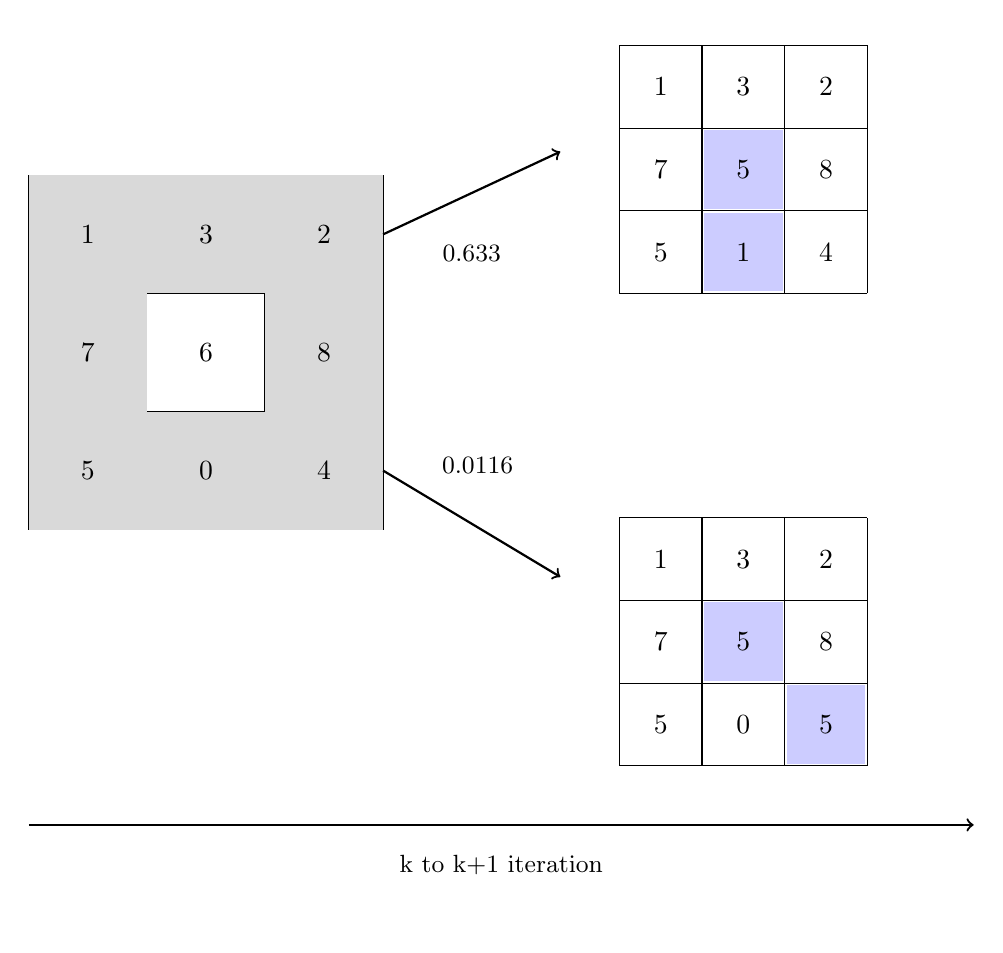
\begin{tikzpicture}[scale=1.5,minimum size=1.5cm]
    \draw (0,0) grid (3,3);
    \node at (0.5,2.5) [fill=gray!30] {1};
    \node at (1.5,2.5) [fill=gray!30] {3};
    \node at (2.5,2.5) [fill=gray!30] {2};
    \node at (0.5,1.5) [fill=gray!30] {7};
    \node at (1.5,1.5) {6};
    \node at (2.5,1.5) [fill=gray!30] {8};
    \node at (0.5,0.5) [fill=gray!30] {5};
    \node at (1.5,0.5) [fill=gray!30] {0};
    \node at (2.5,0.5) [fill=gray!30] {4};
      \draw [->, black, thick] (3.0, 2.5) -- node[below] {\small{0.633}} (4.5, 3.2);
      \draw [->, black, thick] (3.0, 0.5) node[above, shift={(1.2,-0.7)}]{\small{0.0116}} -- (4.5, -0.4);
        \draw [->, black, thick] (0, -2.5) node[below,shift={(6.0,0.25)}]{\small{k to k+1 iteration}} --  (8, -2.5);
         % top branch
        \begin{scope}[shift={(5cm, 2cm)}, scale=0.7]
            \draw (0,0) grid (3,3)   ;
            \node at (0.5,2.5) {1};
            \node at (1.5,2.5) {3};
            \node at (2.5,2.5) {2};
            \node at (0.5,1.5) {7};
            \node at (1.5,1.5) [fill=blue!20, minimum size=1.0cm]{5};
            \node at (2.5,1.5) {8};
            \node at (0.5,0.5) {5};
            \node at (1.5,0.5) [fill=blue!20, minimum size=1.0cm] {1};
            \node at (2.5,0.5) {4};

        \end{scope}
        % Bottom branch
        \begin{scope}[shift={(5cm, -2cm)}, scale=0.7]
            \draw (0,0) grid (3,3)   ;
            \node at (0.5,2.5) {1};
            \node at (1.5,2.5) {3};
            \node at (2.5,2.5) {2};
            \node at (0.5,1.5) {7};
            \node at (1.5,1.5) [fill=blue!20, minimum size=1.0cm]{5};
            \node at (2.5,1.5) {8};
            \node at (0.5,0.5) {5};
            \node at (1.5,0.5) {0};
            \node at (2.5,0.5) [fill=blue!20, minimum size=1.0cm] {5};

        \end{scope}
\end{tikzpicture}
\caption{\small {Possible configurations for the k+1 iteration. Blue cells are the cells whose value changed}}
\label{fig:myfigure3}
\end{figure}
As seen from Figure \ref{fig:myfigure3}, there is a 63.3\% chance that the grid would end up looking like the top and a 1.16\% chance that the grid would look like the bottom in the next iteration. Using this strategy, I can then drift my simulation to be closer to reality.
\pagebreak

\section{Calculating entropy}
Now that a strategy that governs energy movement has been devised, our next task is to find a way to compute entropy. In version 1, a crude method of using bitwise XOR is used. Details on how this is done can be seen within this \href{https://github.com/ShiroHusin/Entropy_Simulation/blob/main/Entropy_Computation.pdf}{document}. However, such a method is not viable when the cells are no longer binary digits. Hence, a new strategy needs to be devised. \par

\vspace{0.3cm}
\noindent
The first step in solving this problem is to look back at the definition of entropy that Ludwig Boltzmann provided. The entropy $S$ is equal to: 
\begin{equation}
    S=k_{b}Ln(\Omega)
    \label{entropy_eq}
\end{equation}
Now the $\Omega$ term is the total number of micro-states or possible configurations that the system can occupy. The challenge is then to find a way to compute $\Omega$. Remembering the \href{https://www.youtube.com/watch?v=mg0hueOyoAw&ab_channel=ParthG}{video} that ParthG made in explaining what entropy is, it became clear that the strategy is to count the number of viable integers combinations that add up a number. \par

\vspace{0.3cm}
\noindent
The technique I decided on is to first, break down the entire square grid into 2x2 sub-matrices. If we let $l$ be equal to the length of the matrix and that $l \in 2\mathbb{Z}$, we would have $\frac{l^2}{4}$ different sub-matrices. In Figure \ref{fig:matrix}, some of the splittings are depicted using arrows and the middle matrix is the grid. Note that the middle matrix is a square matrix, for convenience, it is depicted as a rectangle.

\begin{figure}[H]
  \centering
  \scalebox{1.2}{
    \begin{tikzpicture}[node distance=0.5cm and 0.5cm]
      \node(matrix) {$\begin{bmatrix}
          a_{1,1} & a_{1,2} & \cdots & a_{1,l-1} & a_{1,l} \\
          a_{2,1} & a_{2,2} & \cdots & a_{2,l-2} & a_{2,l} \\
          \vdots  & \vdots  & \vdots & \vdots & \vdots  \\
          a_{l-1,1}& a_{l-1,2} & \ddots &a_{l-1,l-1} & a_{l-1,l}\\
          a_{l,1} & a_{l,2} & \cdots& a_{l,l-1} & a_{l,l}
        \end{bmatrix}$};
        
         \node(submatrix1) [above left=of matrix.north west, xshift=0cm, yshift=1cm] {$\begin{bmatrix}
          a_{1,1} & a_{1,2} \\
          a_{2,1} & a_{2,2}
        \end{bmatrix}$};

         \node(submatrix2) [above right=of matrix.north east, xshift=0cm, yshift=1cm] {$\begin{bmatrix}
          a_{1,l-1} & a_{1,l} \\
          a_{2,l-2} & a_{2,l}
        \end{bmatrix}$};
        
      \node(submatrix3) [below right=of matrix.south west, xshift=-3cm, yshift=-1cm] {$\begin{bmatrix}
          a_{l-1,1} & a_{l-1,2} \\
          a_{l,1} & a_{l,2}
        \end{bmatrix}$};

      \node(submatrix4) [below left=of matrix.south east, xshift=3cm, yshift=-1cm] {$\begin{bmatrix}
          a_{l-1,l-1} & a_{l-1,l} \\
          a_{l,l-1} & a_{l,l}
        \end{bmatrix}$};

        \draw[->, thick] (matrix.north west) -- (submatrix1.south);
        \draw[->, thick] (matrix.north east) -- (submatrix2.south);
      \draw[->, thick] (matrix.south west) -- (submatrix3.north);
      \draw[->, thick] (matrix.south east) -- (submatrix4.north);
    \end{tikzpicture}
  }
  \caption{Submatrix splitting}
  \label{fig:matrix}
\end{figure}

\pagebreak
Now let the grid be called $M$ and its sub-matrices be called $X_{j}$. In this case, $j$ goes from 1 all the way to $\frac{l^2}{4}$. At this point, the next step is $\forall X_{j}$, find the sum of its 4 elements. Now, let the sum of its four elements of each sub-matrix be depicted as $\Phi_{j}$. Remembering the rules of the simulation the sum of its elements or its energy is bounded within: 

$$0\leq \Phi_{j} \leq 32, \;\;\; \Phi_{j} \in \mathbb{Z} $$

Once this is completed, the next step is to find the number of integer combinations of the elements from $X_{j}$, such that its four elements:
\begin{equation}
    a_{j}+b_{j}+c_{j}+d_{j}=\Phi_{j}
    \label{each}
\end{equation}
Where: 
$$a_{j},b_{j},c_{j},d_{j} \in [0,8] \; 	\land \; a_{j},b_{j},c_{j},d_{j} \in \mathbb{Z}$$
\begin{equation}
    \sum_{j=1}^{\frac{l^2}{4}} \Phi_{j} = E
    \label{conservation}
\end{equation}
Now equation \ref{conservation} is the conservation of energy and the simulation is designed such that this is always true. \par

\vspace{0.3cm}
\noindent
Conveniently, there are hundreds of sample codes out there in stack overflow that solve something similar to equation \ref{each}, therefore solving this problem is thankfully not that difficult. The number of possible combinations such that $a_{j}+b_{j}+c_{j}+d_{j}=\Phi_{j}$ is the number of micro-states for each sub-matrix. Lets call this $\omega_{j}$. Some of the calculated values of $\omega_{j}$ corresponding to its $\Phi_{j}$ is shown in the table down below: 
\begin{center}
\begin{tabular}{ |p{4.3cm}|p{3.2cm}|  }
 \hline
Sub-matrix energy ($\Phi_{j}$)& Micro-states ($\omega_{j}$)\\
 \hline
 0 & 1 \\
 1 & 4  \\
 2 & 10 \\
 4 & 35  \\
 6 & 84  \\
 9 & 216  \\
 11 & 324  \\
 14 & 456 \\ 
 16 & 489 \\
\hline
\end{tabular}
\end{center} 
The above table can map $\Phi_{j}$ to its associated $\omega_{j}$ for each sub-matrix $X_{j}$. However, in order to find the total configurations that the grid $M$ can take we have to multiply each of the sub-matrix micro-state where $\Omega$ from equation \ref{entropy_eq} is: 
\begin{equation}
    \Omega=\prod_{j=1}^{\frac{l^2}{4}} \omega_{j}
    \label{Omega}
\end{equation}
For large grids where $l \ge 150$, $\Omega$ becomes a huge number and in some cases, float32 operations in Python may become insufficient. Using the results from equation \ref{Omega} and combining the product rule for logarithms, equation \ref{entropy_eq} can be rewritten as: 
\begin{equation}
    S=k_b\sum_{j=1}^{\frac{l^2}{4}} ln(\omega_{j})
    \label{Total_entropy}
\end{equation}
\vspace{0,3cm}
\noindent
To sum up, while $k\leq I$, and $I$ is the number of iterations. We have:
\begin{figure}[H]
    \centering
    \begin{tikzpicture}[
    SIR/.style={rectangle, draw=red!60, fill=red!5, very thick, minimum size=5mm},
    ]
    %Nodes
    \node[SIR] (Zeroth) {Grid $M$} ;
    \node[SIR]    (First) [below=1.2cm of Zeroth]                              {$\forall a \in M_{k}, \; a \neq 0$};
    \node[SIR]    (Second)    [below=1.2cm of First]       {$F(M_{k},k)$};
    \node[SIR]    (Third)     [below=1.2cm of Second] {$M_{k+1}$};

    \node[SIR] (four) [right=1.2cm of Third]
    {$S(M_{k+1})$};

    \node[SIR] (five) [above=1.2cm of four] {$\omega_{j}$ table} ;

    \node[SIR] (six) [right=1cm of four] {Data-point $(k,S_{k})$} ;
    
    %Lines
    \draw[->, very thick] (Zeroth.south) to node[right] {} (First.north);
    \draw[->, very thick] (First.south)  to node[right] {for each $a$, if $x \sim \mathrm{U}(0,1) <g(c), \;\; U \in \mathbb{R}$} (Second.north);
    \draw[->, very thick] (Second.south)  to node[right] {} (Third.north);
    \draw[->, very thick] (Third.east) to node[right]
    {} (four.west)  ;
    \draw[->, very thick] (five.south) to node[right] {} (four.north) ; 
    \draw[->, very thick] (four.east) to node[right] {} (six.west) ;
    \draw[->, very thick] (Third.west) .. controls  +(left:14mm) and +(left:14mm)   .. node[pos=0.5, left] {$k=k+1$} (Zeroth.west);
    
    \end{tikzpicture}
    \caption{Process or Functional flow diagram}
    \label{fig:my_labels}
\end{figure}
Figure \ref{fig:my_labels} represents a high-level overview of the process steps needed to produce and run the simulation for 1 iteration. $a$ is the elements of the grid/matrix $M$. $U(0,1)$ is a uniform distribution from 0 to 1. $F(M,k)$ is the function responsible for movement, $\omega_{j}$ is the micro-state table, $S(M_{k},k)$ is the entropy function. 